\documentclass[25pt, a0paper, portrait]{tikzposter}
\usepackage[T1]{fontenc}
\renewcommand*\familydefault{\sfdefault}
\usepackage{sfmath}
\usepackage{amsmath}
\usepackage{lipsum}
\usepackage[compress]{cite}
\usepackage{circuitikz}
\usepackage{svg}
\usetikzlibrary{calc} % Add calc library
\usetikzlibrary{positioning, shapes.geometric}

\newcommand{\CORE}{The CORE collaboration}
\newcommand{\PLANCK}{The Planck collaboration}
\newcommand{\prd}{PRD}
\newcommand{\prr}{PRR}
\newcommand{\mnras}{MNRAS}
\newcommand{\jcap}{JCAP}
\newcommand{\jmap}{JMAP}
\newcommand{\joss}{JOSS}
\newcommand{\pasa}{PASA}
\newcommand{\aap}{A\&A}
\newcommand{\prl}{PRL}
\newcommand{\arxiv}{arXiv}

\usepackage[outline]{contour} % glow around text
\contourlength{1.4pt}

% Define the colors and styles
\colorlet{myred}{red!80!black}
\colorlet{myblue}{blue!80!black}
\colorlet{mygreen}{green!60!black}
\colorlet{mydarkblue}{blue!40!black}
\definecolor{lightgray}{RGB}{211,211,211}
\definecolor{varcolor}{RGB}{0,128,0} % Color for specific variables
\colorlet{myorange}{orange!80!black}

\tikzset{
  neuron/.style={
    circle,
    thick,
    draw=myblue,
    minimum size=20pt,  % Adjusted for larger text
    inner sep=0pt,
    outer sep=0pt,
    font=\small,  % Larger text in nodes
  },
  node in/.style={
    neuron,
    draw=mygreen!60!black,
    fill=mygreen!50,
  },
  large hidden/.style={
    neuron,
    minimum size=40pt,  % Adjusted for larger text
    fill=myblue!50,
    font=\Large,  % Larger text in hidden neuron
  },
  node out/.style={
    neuron,
    draw=myred!80!black,
    fill=myred!50,
  },
  connect/.style={
    thick,
    mydarkblue,
  },
  formula box/.style={
    rectangle,
    fill=lightgray,
    inner sep=10pt,
    align=left,
    draw,
    font=\small,  % Larger text in formula box
  },
}


\makeatletter
\renewcommand\TP@maketitle{%
    \centering
    \vspace{-40pt}
    
\includegraphics[height=0.09\textwidth]{reach.png}\hfill
    \begin{minipage}[b]{0.7\linewidth}
        \centering
        \color{titlefgcolor}
        {\Huge \sc \@title \par}
        \vspace*{1em}
        {\huge \@author \par}
        \vspace*{1em}
        {\LARGE \@institute}
    \end{minipage}%
    \hfill
\includegraphics[height=0.09\textwidth]{cambridge-cropped.pdf}
}
\makeatother

\title{Machine learning for radiometer calibration}
\author{Samuel Alan Kossoff Leeney <sakl2@cam.ac.uk>}
\institute{Kavli Institute for Cosmology $\cdot$ Cavendish Laboratory $\cdot$  University of Cambridge}
%\usetheme{Default}
%\usetheme{Rays}
%\usetheme{Basic}
%\usetheme{Simple}
\usetheme{Envelope}
%\usetheme{Wave}
%\usetheme{Board}
%\usetheme{Autumn}
%\usetheme{Desert}

\tikzposterlatexaffectionproofoff{}

\let\oldbibliography\thebibliography
\renewcommand{\thebibliography}[1]{\oldbibliography{#1}
\setlength{\itemsep}{-5pt}} %Reducing spacing in the bibliography.

\pdfinclusioncopyfonts=1 % Fix fonts on non-linux machines

\usepackage{xcolor}
\definecolor{C0}{HTML}{1f77b4}
\definecolor{C1}{HTML}{ff7f0e}
\definecolor{C2}{HTML}{2ca02c}
\definecolor{C3}{HTML}{d62728}
\definecolor{C4}{HTML}{9467bd}
\definecolor{C5}{HTML}{8c564b}
\definecolor{C6}{HTML}{e377c2}
\definecolor{C7}{HTML}{7f7f7f}
\definecolor{C8}{HTML}{bcbd22}
\definecolor{C9}{HTML}{17becf}
\newcommand\C[2][1]{\textcolor{C#1}{#2}}


%\usecolorstyle[colorOne=blue, colorTwo=gray, colorThree=green]{Default}
%\usecolorpalette{BlueGrayOrange}
%\usecolorstyle[colorOne=blue]{mystyle}
%\colorlet{backgroundcolor}{C1}

%% Background Colors
\colorlet{backgroundcolor}{C0!50!white}
\colorlet{framecolor}{black}
%% Title Colors
\colorlet{titlefgcolor}{white}
\colorlet{titlebgcolor}{C0}
%% Block Colors
\colorlet{blocktitlebgcolor}{C0}
\colorlet{blocktitlefgcolor}{white}
\colorlet{blockbodybgcolor}{white}
\colorlet{blockbodyfgcolor}{black}
%% Innerblock Colors
\colorlet{innerblocktitlebgcolor}{C1}
\colorlet{innerblocktitlefgcolor}{black}
\colorlet{innerblockbodybgcolor}{C1!10!white}
%\colorlet{innerblockbodyfgcolor{black}
%% Note colors
\colorlet{notefgcolor}{black}
\colorlet{notebgcolor}{C2!50!white}
\colorlet{notefrcolor}{C2}

\usepackage[hidelinks]{hyperref}
\hypersetup{
    colorlinks,
    linkcolor={C3!50!black},
    citecolor={C0!50!black},
    urlcolor={C0!80!black}
}

\begin{document}
\maketitle

    \block{}{%
        \centering
        
\includegraphics[height=0.09\textwidth]{kicc}
        \hspace{20pt}
        \begin{minipage}[b]{0.73\textwidth}
        We propose a Physics based AI framework for precise radiometer calibration in global 21cm cosmology. These experiments aim to study formation of the first stars and galaxies by detecting the faint 21-cm radio emission from neutral hydrogen. This global or sky-averaged signal is predicted to be five orders of magnitude dimmer than the foregrounds. Therefore detection of the signal requires precise calibration of the instrument receiver, which non-trivially amplifies the signals detected by the antenna. Current analytic methods appear insufficient, causing a major bottleneck in all such experiments. Unlike other methods, our receiver calibration approach is expected to be agnostic to in-field variations in temperature and environment and furthermore does not rely on assumptions that certain critical components are impedance matched. For the first time we propose the use of machine learning for calibration of global 21-cm experiments.
        \end{minipage}%
        \hspace{20pt}
        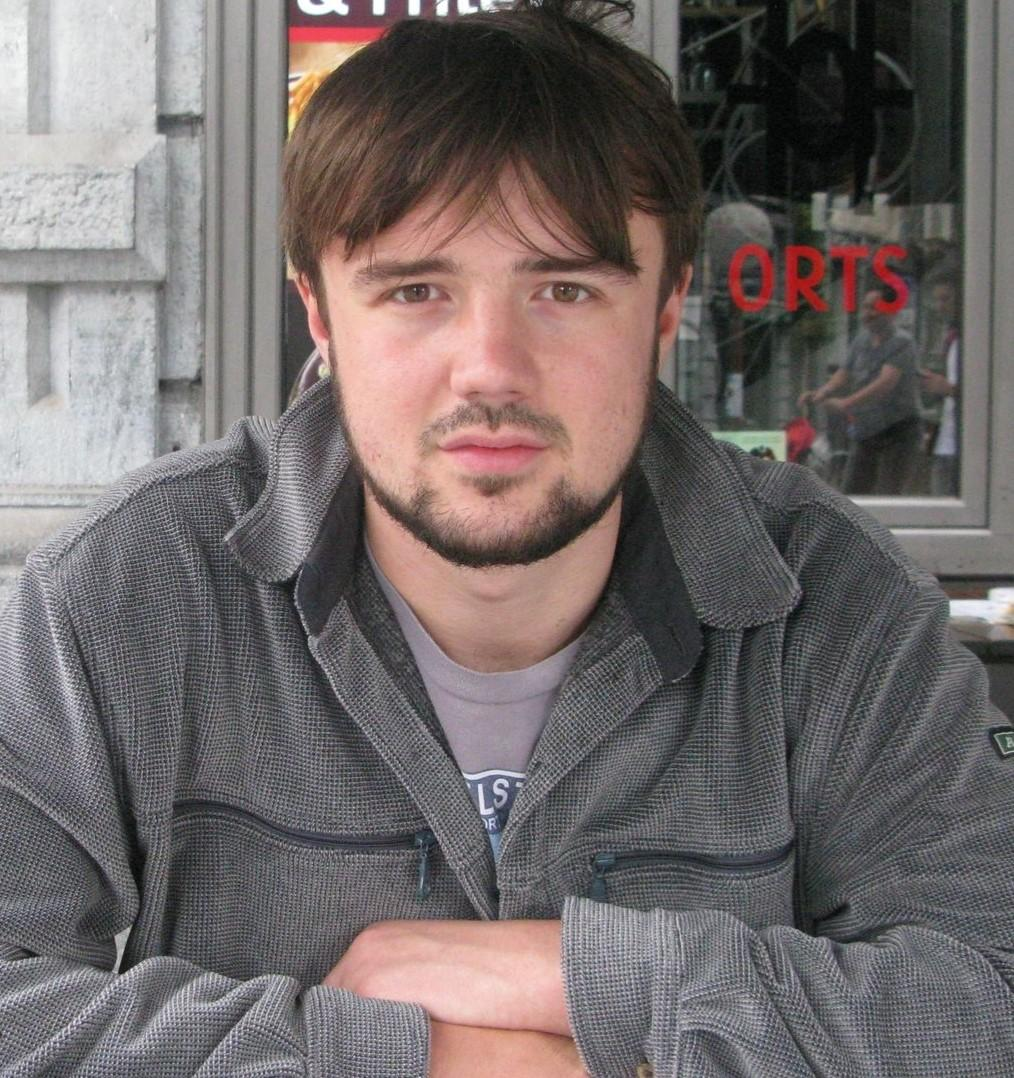
\includegraphics[height=0.09\textwidth]{avatar.jpg}

    }
\begin{columns}
  \column{0.5}


    \block{Global 21cm cosmology}{%

    Cosmologists can study the formation of the first stars by observing radio signals from the early universe emitted by cosmic hydrogen~\cite{pritchard201221}. Observations of the 21cm line could aid our understanding fundamental physics, including the nature of dark matter.
      \begin{tikzfigure}[Predicted 21cm signal.]
        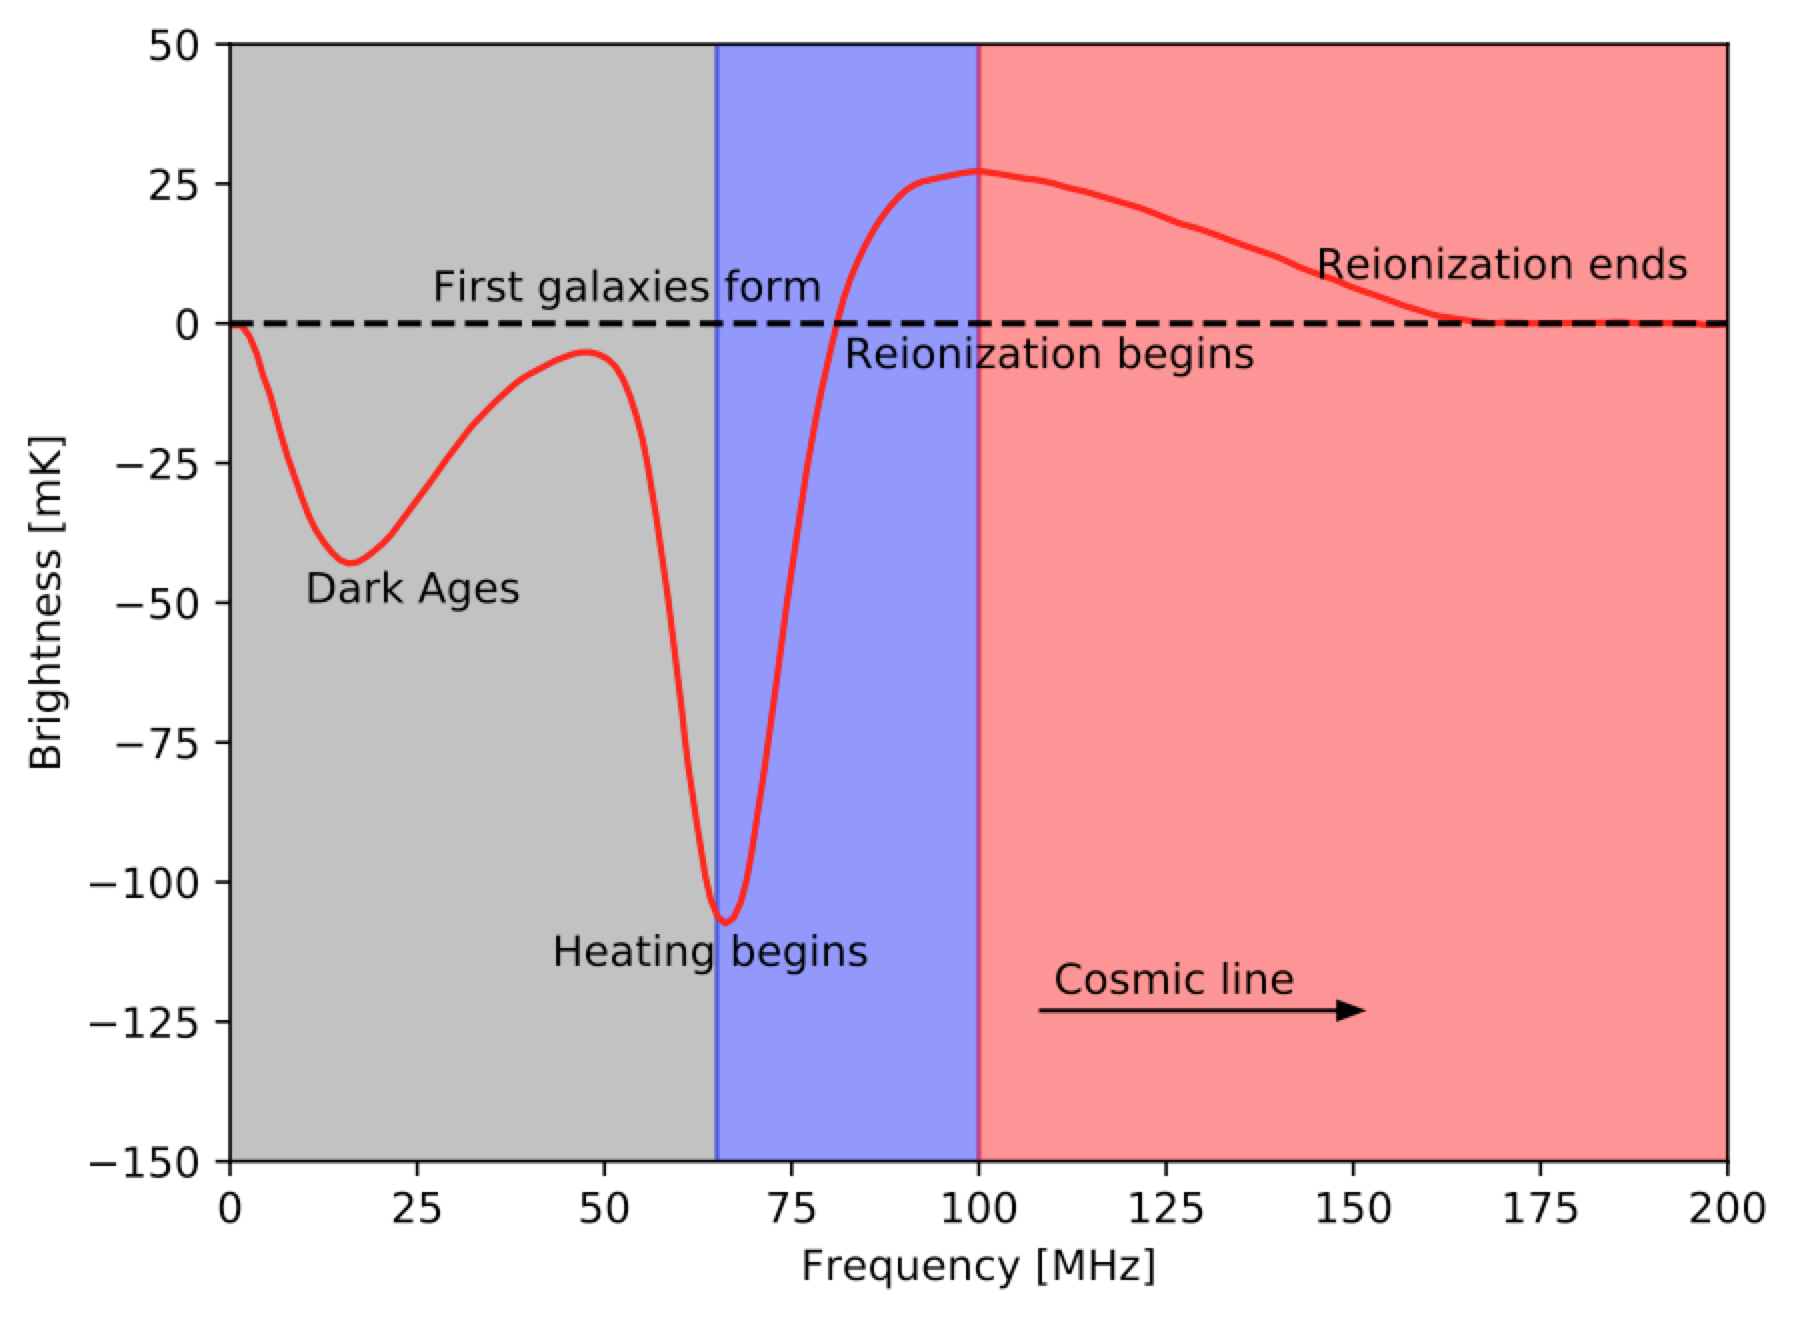
\includegraphics[width=0.2\textwidth]{21cm_signal.png}
        \end{tikzfigure}
        \vspace{0.5em}
        \coloredbox{This can be done with a modestly sized telescope, but calibration of the instrument receiver is particularly challenging. The signal is predicted to be 5 orders of magnitude dimmer than the foreground and because the telescope has a wide, non directional beam it \textbf{cannot target well characterised sources for calibration}.}
        }

    \block{Radiometer calibration}{%
      
      \begin{tikzfigure}[Receiver design, green is 'training/validation data' and blue is the antenna seeing the sky. The system physically switches between the two to train the neural net and then make predictions.]
        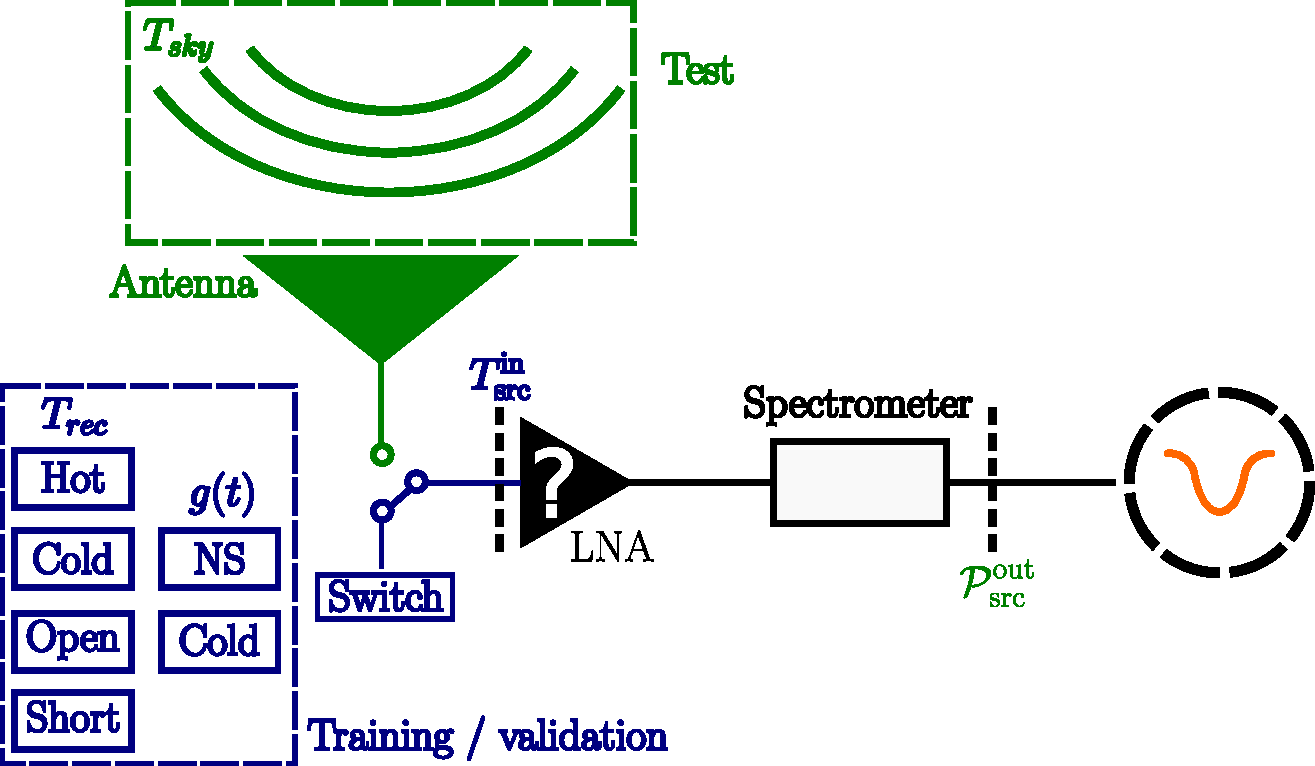
\includegraphics[width=0.45\textwidth]{instrument.pdf}
        \end{tikzfigure}
        \vspace{0.5em}
        The goal of `calibration' is to build a model that links $T^{\text{in}}_{\text{src}}$ to $\mathcal{P}_{\text{src}}^{\text{out}}$. This is challenging because of the non linear time dependent LNA gain $g(t)$ and standing waves created by the unavoidable impedance mismatch between the LNA and the source, described by $T_{rec}$.

        The noise parameter formalism introduced by~\cite{haus1960representation} describes the effect of these standing waves:
        \begin{equation}\label{eq:noise_g}
            \mathcal{P}_{\text{src}}^{out} = gM \bigg( T^{in}_{\text{src}} + T_{min}+T_0\frac{4R_N}{Z_0}\frac{|\Gamma_{\text{src}}-\Gamma_{\text{opt}}|^2}{(1-|\Gamma_{\text{src}}|^2)|1+\Gamma_{\text{opt}}|^2} \bigg).
        \end{equation}

      }


    \block{The case for machine learning}{
        \begin{minipage}{0.19\textwidth}
          \innerblock{No impedance matching}{%
            Typical systems require that components are approximately impedance matched to simplify the noise parameter or noise wave parameter formalisms~\cite{roque2021bayesian}~\cite{monsalve2017calibration}. The ML based method does not rely on these assumptions.
            }
        \end{minipage}\hfill
        \begin{minipage}{0.25\textwidth}
          \innerblock{Maleable to environment}{%
            It is often not possible to build a system that is totally isolated from the external environmental and environmental factors such as system temperature are difficult to model analytically. Neural networks are capable of modeling complex dependencies like this and as such will be useful on future projects, particularly those in space where external temperature is difficult to control.

            }
        \end{minipage}\\
        \vspace{1em}

    }


    % \block{BibTeX}{%
    %     As it is \LaTeX, you can use BibTeX to manage your references. Here is an example of a citation~\cite{2015MNRAS.453.4384H}. You can also use BibTeX to manage the references in the bibliography. Here is a long list: \cite{2014PhRvD..89f3505H, 2015MNRAS.450L..61H, 2015MNRAS.453.4384H, 2016A&A...594A...1P, 2016A&A...594A..20P, 2018A&A...619A..94P, 2018BayAn..13..873H, 2018JCAP...04..016F, 2018JCAP...04..017D, 2018JCAP...04..018C, 2018JCAP...04..019M, 2018JCAP...04..020D, 2018JCAP...04..021B, 2018JCAP...04..022N, 2018JCAP...04..023R, 2018JOSS....3..849H}. You can see these appear in the references section.
    % }
%     \block{Printing your poster}{
% You can print your poster same day (although don't leave it this late!) at the University Print Shop. I recommend a0, portrait, lightweight cloth (which can be gently folded in a suitcase)
%         \href{https://www.pdn.cam.ac.uk/other-pages/avmg/posters}{www.pdn.cam.ac.uk/other-pages/avmg/posters}
%     }





    \column{0.5}

    \block{Network architecture}{

    Predicting antenna temperature (which is the value of interest to cosmologists) directly is not possible as the temperature of the antenna is very different to that of the sources (~5000K). As such we design a system that predicts noise parameters and time dependant gain, all of which are source independent.

    \begin{tikzfigure}[Network architecture and loss function ($\mathcal{L}$). Normalised values highlighted by $\hat{}$.]

      \includesvg[width=0.42\textwidth]{nn.svg}
          \end{tikzfigure}

    }
    \block{Results}{
      Results when network trained on a simulation of the REACH~\cite{de2019reach}~\cite{razavi2023receiver} receiver. More calibration sources are used than is standard to provide extra information on the effect of the impedance mismatch between the antenna and the LNA.
        \begin{tikzfigure}[Testing on the simulated REACH receiver with realistic power law antenna.]
            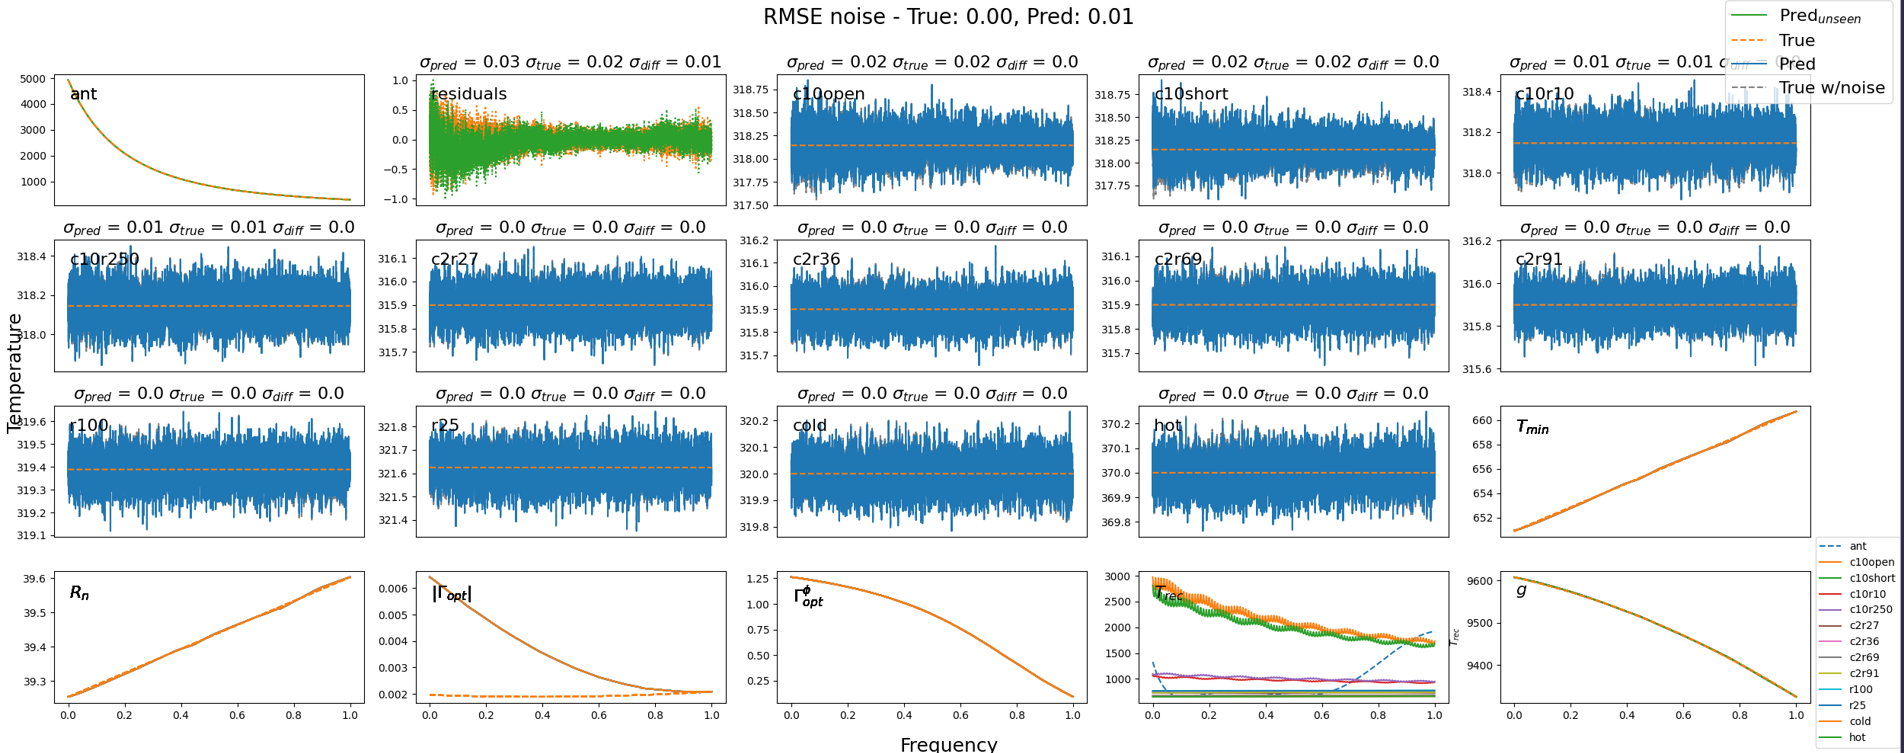
\includegraphics[height=0.16\textwidth]{placeholder_results.png}%
          \end{tikzfigure}
          }

    \block{Conclusion}{%
      Our system generates training data for the neural network by physically switching between sources representative of the antenna. It is capable of highly sensitive calibration on realistic simulated data. It is novel in that it does not rely on any assumptions about impedance matching. These methods will be tested in the near future in field. Furthermore, the ML based methods we propose are designed to work with existing instrumentation. In the future the process should be inverted so that system design is motivated by statistical methods.

    }

    \renewcommand{\section}[2]{}%
    \block{References}{%
        \begin{minipage}[b]{0.35\textwidth}
          \bibliographystyle{unsrt}
            \tiny
            \bibliography{template_poster}
        \end{minipage}%
        
\includegraphics[width=0.1\textwidth]{QR.png}
    }

    \note[targetoffsetx=0.18\textwidth,targetoffsety=0.02\textwidth, connection,angle=135,radius=0.08\textwidth]{Repository with source files for slides, poster and contact info.}
\end{columns}
\end{document}
